\begin{figure*}[!hbtp]
  \centering

  \subfloat{
    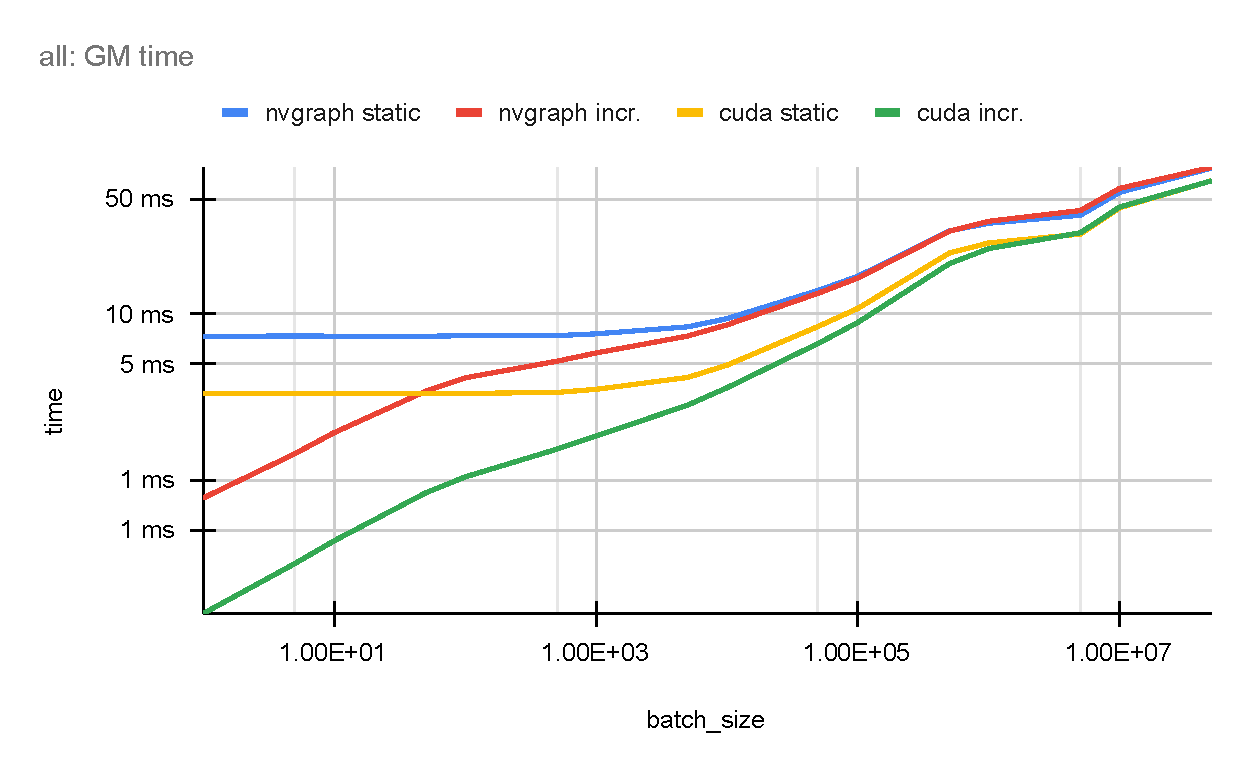
\includegraphics[width=0.48\textwidth]{out/pr-cuda-st-vs-it-time.pdf}
    \label{fig:pr-cuda-st-vs-it-time}
  }
  \subfloat{
    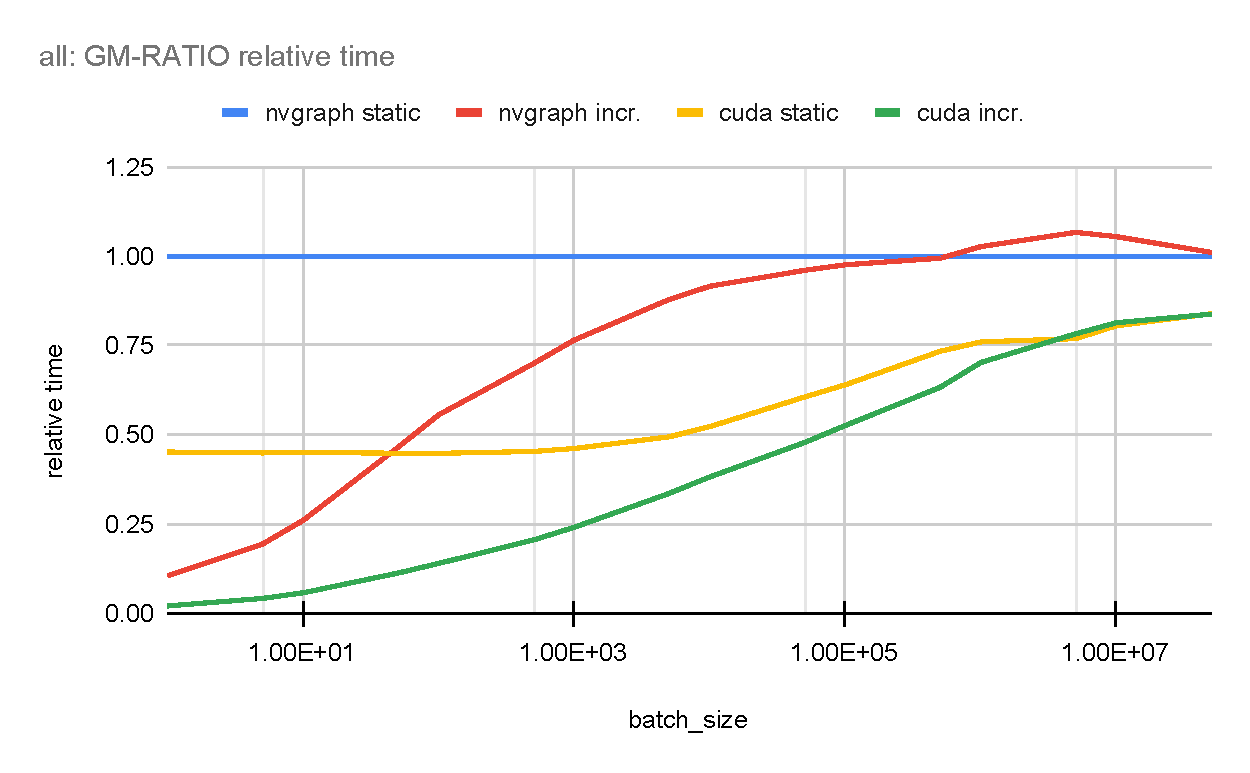
\includegraphics[width=0.48\textwidth]{out/pr-cuda-st-vs-it-rtime.pdf}
    \label{fig:pr-cuda-st-vs-it-rtime}
  }

  \caption{GM time taken for static and incremental PageRank with nvGraph and CUDA implementation, with respect to nvGraph’s static PageRank is shown on the left. Relative GM time taken is shown on the right. This is done on seven temporal graphs. Error measurement between the previous and current iteration is done using L1-norm except for nvGraph, which uses L2-norm instead. Batch sizes range from $10^0$ to $5 * 10^7$.}
  \label{fig:pr-cuda-st-vs-it}
\end{figure*}
